\documentclass[11pt,a4j]{jreport}
\usepackage[japanese]{babel}
\usepackage[top=30truemm,bottom=30truemm,left=25truemm,right=25truemm]{geometry}

\usepackage{algorithmic}
\usepackage{amsmath,amssymb,amsfonts}
\usepackage{bm}
\usepackage{cite}
\usepackage{color}
\usepackage{colortbl}
\usepackage{comment}
\usepackage{fancyhdr}
\usepackage{float}
\usepackage[dvipdfmx]{graphicx}
\usepackage[dvipdfmx]{hyperref}
\usepackage{lscape}
\usepackage{multicol}
\usepackage{multirow}
\usepackage[dvipdfmx]{pict2e}
\usepackage[ipaex]{pxchfon}
\usepackage{pxjahyper}
\usepackage{tabularx}
\usepackage{textcomp}
\usepackage{ulem}
\usepackage{underscore}
\usepackage{url}
\usepackage{wrapfig}
\usepackage{xcolor}

\hypersetup{
	colorlinks=false, % リンクに色をつけない設定
	bookmarks=true, % 以下ブックマークに関する設定
	bookmarksnumbered=true,
	pdfborder={0 0 0},
	bookmarkstype=toc
}

\setlength{\headheight}{15.5pt}

\begin{document}

\thispagestyle{empty}
\begin{center}
    \vspace{20mm}
    {\Large\noindent 令和5年度 卒業論文 (準学士) 論文番号12} \\
    \vspace{40mm}
    {\Huge\noindent\textbf{Text-to-Videoモデルを用いて生成された動画に対する定量的評価指標の検討とその評価}}\\
    \medskip
    %{\huge\noindent\textbf{論文タイトル(2行目)}}
    %\vspace{\baselineskip}
    {\Large\noindent\textbf{Study and Evaluation of Quantitative Evaluation Metrics for Videos Generated by Text-to-Video Model.}}\\
    %\medskip
    %{\large\noindent\textbf{英語title(2行目)}}\\
    \vspace{40mm}
    {
        \Large\noindent
        2024年2月15日
        \vspace{\baselineskip}
        一関工業高等専門学校\\
        未来創造工学科 情報・ソフトウェア系 \\
        \vspace{\baselineskip}
        村上研究室 \\
        f19135 本田涼大\\
        Suzuto Honda \\
        \vspace{\baselineskip}
        主査 村上力    \\
        副査 千田栄幸 \\
        副査 小保方幸次 
    }
    \vspace{40mm}
\end{center}

\thispagestyle{empty}
\newpage

\renewcommand{\abstractname}{要旨}
\begin{abstract}
    近年動画像生成分野が目覚ましい発展を見せている.オープンソースかつ個人のコンピュータでも十分に利用できるほど軽量な,新たなモデルや LoRA \cite{hu2021lora} が次々に登場している.しかし,動画像生成モデルに対する評価指標に関する研究は殆ど行われてきていない.特に,Text-to-Video モデルにおけるプロンプトと生成動画像の関連性に対する評価指標においては,人間の行う評価との高い相関があることが示された手法が存在していない.既存手法である CLIPScore \cite{hessel2021clipscore} においても高い相関が確認されているわけではない.
    
    そこで,プロンプトと生成動画像の関連性に対する評価指標として,動画像キャプション生成モデルを用いて生成動画像に対するキャプションを取得し,文書埋込みモデルを用いてプロンプトとキャプションを比較した結果をプロンプトに対する動画像の追従度とする手法を提案する.本論文では,その評価指標としての有効性を検証する.
    
    複数のキャプション生成モデル及び文書埋込みモデルの組み合わせについて検証した結果,提案手法と人間の評価との間に高い相関は確認されず,CLIPScore と比較しても大きな差がないことが分かった.
\end{abstract}
\renewcommand{\abstractname}{Abstract}
\begin{abstract}
    Nowadays, the development of Video Generation has been remarkable. New models and LoRAs appear one after another that are open source and light enough to be used on personal computers. However, there has been little research on evaluation indices for the video generation models. In particular, no method has been shown to correlate highly with human evaluations of the relationship between prompts and generated videos in the Text-to-Video model. The CLIPScore, an existing method, does not show a high correlation.
    
    We propose a method to evaluate the relationship between a prompt and a generated video image by acquiring a caption for the generated video image using a video caption generation model and comparing the result of the comparison between the prompt and the caption using a text embedding model as a measure of the video image following to the prompt. This paper examines its effectiveness as an evaluation indicator.
    
    The validation of several combinations of caption generation and language embedding models showed no high correlation between the proposed method and human evaluation, and there was no significant difference compared to CLIPScore.
\end{abstract}

\tableofcontents
\listoffigures
\listoftables
%\lstlistoflistings

\pagestyle{fancy}
\lhead{\rightmark}
\renewcommand{\chaptermark}[1]{\markboth{第\ \normalfont\thechapter\ 章~~#1}{}}

\chapter{はじめに}
\label{intro}

\section{研究の背景}

近年,俗に生成AIと呼ばれる深層学習を用いたテキスト生成モデルや画像生成モデルが大きな発展を見せている.画像生成モデルである StableDiffusion \cite{rombach2022high} などが様々な分野で活躍している.特に動画像生成分野においては,StableDiffusion をもとに開発された Text-to-Video (以下 T2V)モデルであるAnimateDiff \cite{guo2023animatediff} や,イラストや写真内に写る人物に指定した動きをさせることができる Animate Anyone \cite{hu2023animate} などの高性能なモデルが次々に登場している.

しかしながら,動画像生成分野においては評価指標の研究はそれほど盛んではない.T2V モデルに関するどの論文も定性的な評価のみを掲載し,定量的な評価については言及しないことが殆どである.数少ない T2V モデルに対する評価指標の1つである EvalCrafter \cite{liu2023evalcrafter} では動画像生成モデルに対する評価を「映像の品質」「プロンプトと動画の関連性」「動き方の自然さ」「隣接フレーム間の整合性」の4つの観点から行っているが,いずれも人間の評価との相関は非常に高いとはいえず,十分な性能ではない.特に「プロンプトと動画の関係性」に関しては,現在 CLIPScore \cite{hessel2021clipscore} が主に使われているが,他の分野と比較して人間の評価との相関が最も低く,十分な性能があるとはいえない.要因として以下のことが考えられる.

\begin{quote}\begin{itemize}
    \item CLIP \cite{radford2021clip} は一般的な画像に対して有効であるため,類似したスタイルの画像に対して正確に評価することができない可能性がある.
    \item 昨今の動画像生成モデルは品質の高い動画像を生成できることが多く,品質が高いというだけでプロンプトからの埋込み空間内での距離が大きく動かず,スコアにプロンプトの追従度が反映されにくくなっている可能性がある.
    \item 上記とは逆に,意味的に近いにも拘らず埋込み空間内での距離が近くならない可能性があり,そうした場合に意図せず追従度が低く算出されてしまう.
\end{itemize}\end{quote}

ある分野において評価指標が誕生することは,性能の比較様々な観点からの比較や,モデルの利点や欠点を明確にすることが可能になることを意味する.EvalCrafter において最も人間の評価との相関が低かった分野である「プロンプトと動画の関係性」を評価する指標を新たに考案することにより,T2V モデルのさらなる発展を望むことができると考える.

\section{研究の目的}

本研究では,T2V モデルにおけるプロンプトに対する動画像の追従度の新たな評価指標を提案し,提案手法がどれほどの有効性を持つのかを検証する.

\section{本論文の構成}
本論文の構成は以下の通りである.

第 \ref{related-works} 章では,EvalCrafter や CLIPScore などの本研究に関連した研究を紹介する.第 \ref{our-method} 章では提案手法の概要や求めるものについて説明を行う.第 \ref{experiment} 章では提案手法の出したスコアと人間の評価の相関を計算し,既存手法と比較する.第 \ref{conclusion} 章では論文全体のまとめと今後の展望を記述する.

\chapter{関連研究}
\label{related-works}
\section{EvalCrafter}
\label{sec:evalcrafter}

本研究の先行研究には EvalCrafter \cite{liu2023evalcrafter} がある.EvalCrafter は,動画像生成モデルを多角的に評価するために様々な指標を組み合わせたものである.第\ref{intro}章に記述したように,動画像生成モデルに対する評価指標を4つの分野に分けており,それぞれについて人間の行った評価との相関係数の値が記述してある.「映像の品質」「隣接フレーム間の整合性」については中程度の相関がみられたが,「プロンプトと動画の関連性」「動き方の自然さ」については高い相関が得られなかった.

\section{CLIPScore}
\label{sec:clipscore}

\begin{figure}[t]
    \centering
    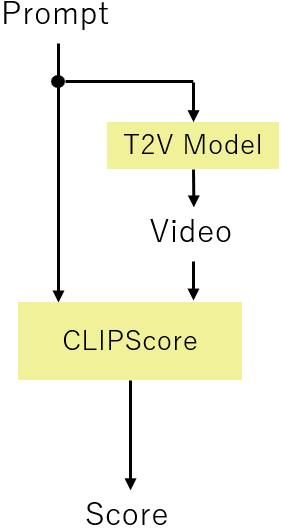
\includegraphics[width=0.3\linewidth]{CLIPScore.png}
    \caption{CLIPScore を用いたプロンプトに対する画像の追従度算出}
    \label{fig:CLIPScore}
\end{figure}

CLIPScore \cite{hessel2021clipscore} は,CLIP \cite{radford2021clip} というテキスト及び画像データを同じ埋め込み空間に置くモデルを用いて,テキストと画像の類似度を算出するモデルである.図 \ref{fig:CLIPScore} のように,プロンプト及び動画像をモデルに入力として与えることでプロンプトに対する動画像の追従度が算出される.画像 $i$ とそのプロンプト $p$ に対して,$w=2.5$ として,埋込みを $\text{emb}(\cdot$) としたとき,CLIPScoreは次のように計算する.

\begin{equation}\text{CLIP-S}(p,i)=w\cdot\max(\cos(\text{emb}(p),\text{emb}(i)),0)\end{equation}
\label{eq:CLIPScore}

生成された動画を $V$ ,その各フレームを $v_t$ 動画のフレーム数を $N$ とする.動画像に対してCLIPScoreを計算するとき,最終的なスコアはすべてのフレームの個々のスコアの平均によって導かれる.

\section{T2Vモデル}
\label{sec:t2v}

本稿では T2V モデルとしてAnimateDiff \cite{guo2023animatediff} を実験に使用する.AnimateDiff は Text-to-Image (以下 T2I) モデルである StableDiffusion \cite{rombach2022high} を動画像出力のために拡張したモデルである.特徴的な点として,大規模な動画データセットを用いて汎化性能の高いモーションモデリングモジュールに時間的な連続性を別途学習させる点がある.このモーションモデリングモジュールを StableDiffusion に適用することで,生成されるフレーム間の動きの滑らかさと一貫性を与え,事前に学習していた重みを保持しつつ動画像出力に適応させることを可能にした.

\section{キャプション生成モデル}
\label{sec:caption}

キャプション生成モデルは一般に動画像を処理するエンコーダ部とキャプションへと変換するデコーダ部からなる.今回使用したモデルはエンコーダ部に Vision Transformer \cite{dosovitskiy2020vit} を用いているもの \cite{vit+gpt2} と TimeSformer \cite{Bertasius2021tsf} を用いているもの \cite{tsf+gpt2} の2つである.デコーダ部は GPT2 \cite{radford2019gpt2} で共通している.いずれも Huggingface \footnote{Hugging Face – The AI community building the future. \url{https://huggingface.co/}}から学習済みのパラメータを含んだチェックポイントが取得可能である.

Vision Transformer は, Transformer \cite{vaswani2017transformer} のエンコーダ部分を用いて画像パッチを単語のように読み込むことで非常に高性能な画像のエンコードが可能なモデルである.TimeSformer は,動画を時間軸アテンション及び空間軸アテンションの2種のパッチを適用させ,画像と同様にTransformerに認識させる機能を持つ.

デコーダに用いられているGPT2も基本的にはTransformerと同様の構造を持つ.特定のタスクに特化した学習は行わず,代わりに大きな言語モデルを事前学習させることにより,zero-shot での高い性能を誇る.

\section{文書埋込みモデル}
\label{sec:emb}

本稿では文書埋込みモデルとしてBERT \cite{devlin2018bert} とE5 \cite{wang2022e5} を採用した.

BERT (Bidirectional Encoder Representations from Transformers, Transformer による双方向エンコーダ) はGoogleから発表された文書埋込みモデルである.文章を文頭と文末から双方向に学習するように設計されており,それにより学習していない単語の意味を類推できる.E5(EmbEddings from bidirEctional Encoder rEpresentation,双方向エンコーダ表現からの埋込み) はredditやwikipediaから収集した大規模なテキストと画像のペアのデータセットを用いて対照学習を行った後に高品質なデータセットで学習を行っている.

\chapter{提案手法}
\label{our-method}

\begin{figure}[ht]
    \centering
    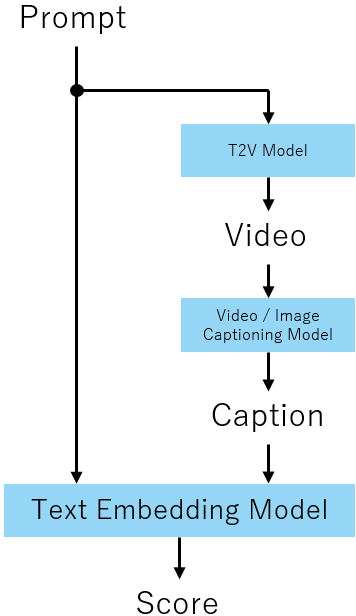
\includegraphics[width=0.3\linewidth]{OurMethod.png}
    \caption{提案手法による追従度の評価}
    \label{fig:OurMethod}
\end{figure}

T2V モデルはプロンプトと呼ばれる入力指示文からに従い動画を生成する.動画キャプションモデルは動画を元に説明文を作成する.ここにはいくつか評価指標があり,高精度でキャプションが作成できることがわかっている.従って,図 \ref{fig:OurMethod} のように動画に対し生成したキャプションがプロンプトと意味的にどれだけ近いのかを評価することでプロンプトへの動画の追従度を評価することができると仮定する.一度テキストに変換してから比較を行うため,画像中の物体などの画風でない情報が強調され,予想される既存手法の問題点である「類似したスタイルの画像に対して正確な評価ができない」という点や「美麗な画像同士では距離が大きく動かないためにスコアが変化しにくい」という点に対して改善が見込める.

EvalCrafter \cite{liu2023evalcrafter} ではプロンプトに対する動画の追従度に関する指標として CLIPScore \cite{hessel2021clipscore} 以外にもいくつか提案されている.しかし,そのいずれも CLIPScore よりも性能が低いか,特定の画像に対してのみ有効である.一般的な画像に対して使用可能である手法の中で最も性能が高い CLIPScore を提案手法の比較対象とする.

パラメータ $\theta$ を持つ文書埋込みモデルを$\rm{emb}_\Theta(\cdot)$,プロンプトを$p$,キャプションを$c$とするとき,例えばプロンプトの埋込みは$\rm{emb}_\Theta(p)$で表される.生成された動画のプロンプトへの追従度を以下のように定める.この値の値域は-1~1である.

\begin{equation}\cos(p,c;\Theta)=\frac{\rm{emb}_\Theta(p)\cdot \rm{emb}_\Theta(c)}{\|\rm{emb}_\Theta(p)\|\;\|\rm{emb}_\Theta(c)\|}\end{equation}
\label{eq:cos}

\chapter{性能評価}
\label{experiment}
\section{概要}

提案手法の有効性を評価するために,AnimateDiff を用いて生成した動画像31本に対し,提案手法により出力したスコアとアンケートの結果から得た評価の相関を見る.また,従来手法として CLIPScore \cite{hessel2021clipscore} を用いた場合の人間の評価との相関も算出する.

実験に使用するプロンプトと動画像のペアを作成する.プロンプトは EvalCrafter \cite{liu2023evalcrafter} のリポジトリに置かれている700のプロンプトの中から無作為に抽出した.動画像生成にはAnimateDiff \cite{guo2023animatediff} を使用した.このとき, モデルのファインチューニングに用いるLoRA(Low-Rank Adaption,低ランク適用) \cite{hu2021lora} は AnimateDiff の GitHub リポジトリ \footnote{guoyww/AnimateDiff: Official implementation of AnimateDiff. \url{https://github.com/guoyww/AnimateDiff}} 内に存在する bash ファイルからダウンロードできる ToonYou\footnote{ToonYou - Beta 6 ★|Stable Diffusion Checkpoint|Civitai \url{https://civitai.com/models/30240/toonyou}},Lyriel\footnote{Lyriel - v1.6|Stable Diffusion Checkpoint|Civitai \url{https://civitai.com/models/22922?modelVersionId=72396}},Rcnz Cartoon 3d\footnote{RCNZ Cartoon 3d - v2.0|Stable Diffusion Checkpoint|Civitai \url{https://civitai.com/models/66347/rcnz-cartoon-3d}},majicMIX realistic\footnote{majicMIX realistic 麦橘写実 - v5 preview|Stable Diffusion Checkpoint|Civitai \url{https://civitai.com/models/43331?modelVersionId=79068}},Realistic Vision V6.0 B1\footnote{Realistic Vision V6.0 B1 - V5.1 (VAE)|Stable Diffusion Checkpoint|Civitai \url{https://civitai.com/models/4201?modelVersionId=130072}},Tusun\footnote{LEOSAM's TuSun/Pallas's cat/manul/マヌルネコ LoRA - v4.0|Stable Diffusion LoRA|Civitai \url{https://civitai.com/models/33194?modelVersionId=97261}}$^,$\footnote{LEOSAM's HelloWorld XL - Reality2.0|Stable Diffusion Checkpoint|Civitai \url{https://civitai.com/models/43977?modelVersionId=50705}},FilmVelvia\footnote{LEOSAM's FilmGirl 膠片机 Film Grain LoRA \& LoHA - VELVIA 2.0 LoRA|Stable Diffusion LoRA|Civitai \url{https://civitai.com/models/33208?modelVersionId=90115}}$^,$\footnote{majicMIX realistic 麦橘写実 - v5 preview|Stable Diffusion Checkpoint|Civitai \url{https://civitai.com/models/43331?modelVersionId=55911}},GhibliBackground\footnote{(Pyramid)_lora_Ghibli_Background - v1.0|Stable Diffusion LoRA|Civitai \url{https://civitai.com/models/64610/pyramidloraghiblibackground}}$^,$\footnote{Counterfeit-V3.0 - v3.0|Stable Diffusion Checkpoint|Civitai \url{https://civitai.com/models/4468?modelVersionId=57618}} の8つを使用した.生成された動画はすべて秒間8フレーム,全体12フレームの2秒の動画で,解像度は512$\times$512である.

次に,生成された動画像に対してキャプションを生成する.動画キャプションモデルの性能比較のため,キャプション生成は ViT+GPT2 \cite{vit+gpt2} と TSF+GPT2 \cite{tsf+gpt2} の2つのモデルを用いて行った.

最後に各動画像のプロンプトと生成されたキャプションを文書埋込みモデルを用いてプロンプトへの動画像の追従度を算出し,人間の評価との相関をCLIPScoreを用いたときの相関と比較する.

\section{アンケート}

アンケートでは,生成した動画像とそのプロンプトに対して人間による評価を行った. 31組の動画像とプロンプトのペアに対し,被験者21人に「1. 動画に対する簡単な説明」「2. 動画像がプロンプトに従っているかの5段階評価」「3. 動画像の総合的な品質の5段階評価」を質問した.ただし,被験者が回答について相談などすることがないよう,対面にてアンケートを行った.アンケートは Google Forms により作成した.質問1に回答する前に質問2に記述されているプロンプトが目に入らないように間に改ページを挟み,すべての回答欄を必須フィールドにしている.質問した3問のうち,質問2は手法の評価に使用した.質問1と3は今回は使用することはなかった.

\section{実験環境}

実験環境1(AnimateDiffによる動画像生成)

\begin{quote}\begin{itemize}
    \item OS: Ubuntu 22.04.3 LTS
    \item CPU: 12th Gen Intel(R) Core(TM) i5-12600K
    \item RAM: DDR4-2666 64GB (16GBx4)
    \item GPU: NVIDIA GeForce RTX 3060 12GB
    \item Python 3.10.13, Anaconda 23.11.0, PyTorch 1.13.1
\end{itemize}\end{quote}

実験環境2(上記以外)

\begin{quote}\begin{itemize}
    \item OS: Windows 11 Home 64bit 22H2 (OS Build 22621.3007)
    \item CPU: 11th Gen Intel(R) Core(TM) i7-11800H
    \item RAM: DDR4-3200 16GB (8GBx2)
    \item GPU: NVIDIA GeForce RTX 3060 Laptop GPU
    \item Python 3.10.11, PyTorch 1.13.1
\end{itemize}\end{quote}

\section{結果}


%\begin{minipage}{1\linewidth}
\begin{table}[ht]
    \centering
    \caption{\textbf{提案手法のスコアと人間の評価の相関}}
    $\rho,\phi$ はそれぞれスピアマン相関とケンドール相関を表す.
    \begin{tabular}{c|l|c|l|rr}
        &\textbf{モデル名} & \textbf{入力} & \textbf{文書埋込みモデル} & $\rho$ & $\phi$ \\
        %&\textbf{モデル名} & \textbf{入力} & \textbf{文書埋込みモデル} & $\rho$ & $\phi$ \\
        \hline\hline
        既存手法&\begin{tabular}{l}CLIPScore \cite{hessel2021clipscore}\end{tabular}&動画&-&-0.1881&-0.1306\\
        \hline\hline
        \multirow{10}{*}{提案手法}&\multirow{2}{*}{\begin{tabular}{l}TimeSformer-GPT2\\Video Captioning \cite{tsf+gpt2}\end{tabular}}&\multirow{2}{*}{動画}&E5 \cite{wang2022e5}&0.1356&0.1088\\\cline{4-6}
        &&&BERT \cite{devlin2018bert}&\textbf{0.2176}&\textbf{0.1611}\\
        \cline{2-6}
        &\multirow{8}{*}{\begin{tabular}{l}ViT-GPT2 Image\\Captioning \cite{vit+gpt2}\end{tabular}}&\multirow{2}{*}{動画}&E5&-0.2717&-0.2046\\\cline{4-6}
        &&&BERT&-0.2556&-0.1828\\\cline{3-6}
        &&\multirow{2}{*}{画像(平均)}&E5&-0.2557&-0.1915\\\cline{4-6}
        &&&BERT&-0.2981&-0.1959\\\cline{3-6}
        &&\multirow{2}{*}{画像(最高)}&E5&-0.1425&-0.1132\\\cline{4-6}
        &&&BERT&-0.1786&-0.1349\\\cline{3-6}
        &&\multirow{2}{*}{画像(最低)}&E5&\textbf{-0.3819}&\textbf{-0.2742}\\\cline{4-6}
        &&&BERT&-0.3569&-0.2655\\
    \end{tabular}
    \label{tab:corr}
\end{table}

%\end{minipage}

実験結果を表\ref{tab:corr}及び表\ref{tab:score}に示す.ただし,表\ref{tab:corr}中において,「入力」列にはそのモデルに動画形式で入力したか画像形式で入力したかを記述している.画像形式で入力した場合,各画像のスコアの平均・最高値・最低値を記録した場合でそれぞれ場合分けしている.また,$\rho$はスフィアマン相関,$\phi$はケンドール相関を示す.

ほとんどの組み合わせにおいて無相関または負の弱い相関を記録した.スピアマン相関・ケンドール相関共に,TimeSformer-GPT2 Video Captioning \cite{tsf+gpt2} と BERT \cite{devlin2018bert} の組み合わせが最も Ground-truth との相関が高く(図\ref{fig:vid-corr}),1フレームずつ入力して最低値を採用したときの ViT-GPT2 Image Captioning \cite{vit+gpt2} と E5 \cite{wang2022e5} の組み合わせが Ground-truth との相関係数の絶対値が最も高い結果となった(図\ref{fig:min-corr}).

出力されたスコアに着目すると,ほとんどの動画像に対して CLIPScore \cite{hessel2021clipscore} 及び TimeSformer-GPT2 Video Captioning は 0.20 ~ 0.40 の値を記録し,ViT-GPT2 Image Captioning では 0.70 ~ 0.80 の値を記録した.

プロンプトに着目すると,TimeSformer-GPT2 Video Captioning により生成されたキャプションは「A person」等の人間を指す言葉から始まっている.これは抜粋した部分に限らず,すべてのキャプションに対して見られた.

\begin{comment}
\begin{figure}[t]
    \centering
    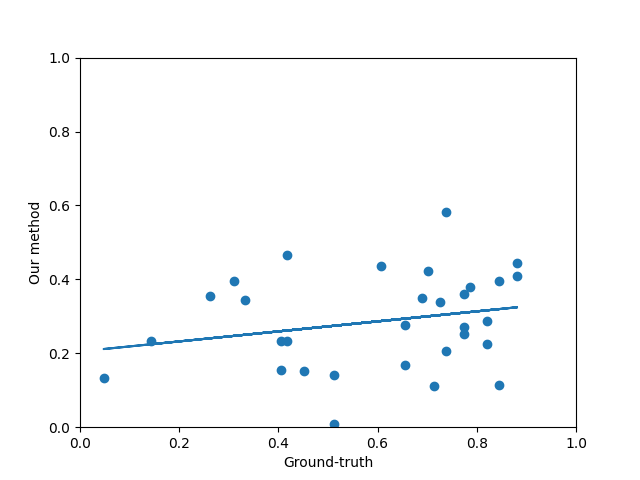
\includegraphics[width=0.5\linewidth]{vid_corr.png}
    \caption{TimeSformer-GPT2 Image Captioning と BERT を用いたスコアと Ground-truth の散布図}
    \label{fig:vid-corr}
\end{figure}

\begin{figure}[t]
    \centering
    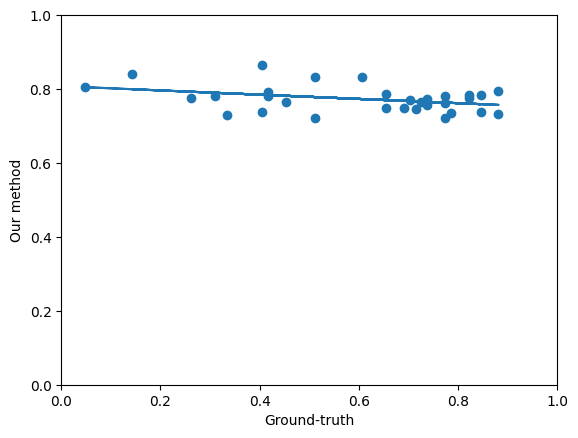
\includegraphics[width=0.5\linewidth]{min_corr.png}
    \caption{ViT-GPT2 Image Captioning(画像入力,最小値採用) と E5 を用いたスコアと Ground-truth の散布図}
    \label{fig:min-corr}
\end{figure}
\end{comment}

\begin{figure}[ht]
    \centering
    % 左の図
    \begin{minipage}[c]{0.5\hsize}
        \centering
        \label{tab:leftfigure}
        % ここに画像の挿入
        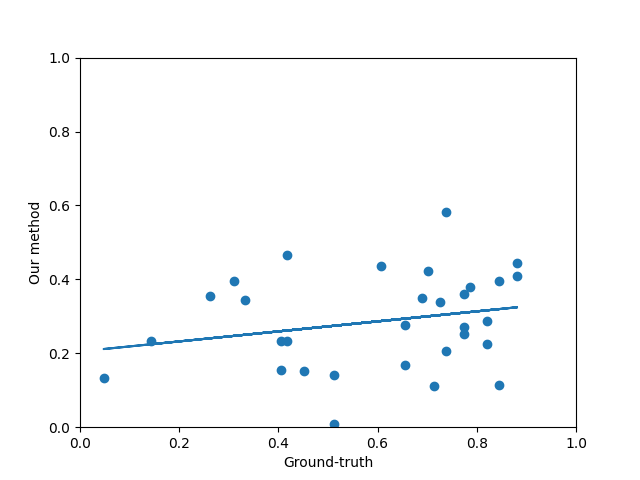
\includegraphics[width=\linewidth]{vid_corr.png}
        \caption{TimeSformer-GPT2 Image Captioning と BERT を用いたスコアと Ground-truth の散布図}
        \label{fig:vid-corr}
    \end{minipage}
    % 右の図
    \begin{minipage}[c]{0.45\hsize}
        \centering
        \label{tab:rightfigure}
        % ここに画像の挿入
        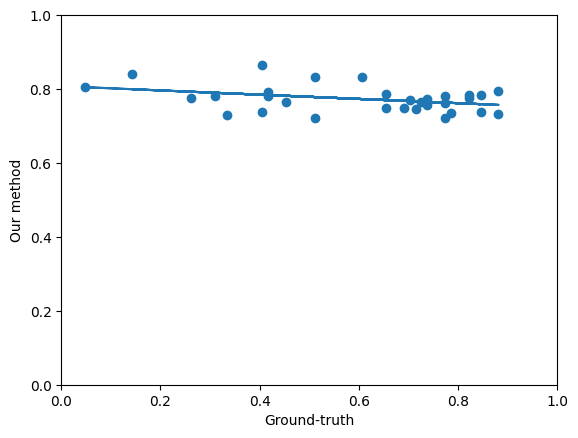
\includegraphics[width=\linewidth]{min_corr.png}
        \caption{ViT-GPT2 Image Captioning(画像入力,最小値採用) と E5 を用いたスコアと Ground-truth の散布図}
        \label{fig:min-corr}
    \end{minipage}
\end{figure}

\begin{landscape}
    \begin{table}
        \centering
        \caption{\textbf{各モデルのキャプションとスコア }(抜粋)}
        \begin{tabular}{r|r|c|c|c|c}
            \multicolumn{2}{r|}{\scriptsize{動画像のサムネイル}} & 
                \begin{minipage}{20mm}\centering\scalebox{0.1}{\includegraphics{IMAGE/1-1-1.eps}}\end{minipage} &
                \begin{minipage}{20mm}\centering\scalebox{0.1}{\includegraphics{IMAGE/1-2-1.eps}}\end{minipage} &
                \begin{minipage}{20mm}\centering\scalebox{0.1}{\includegraphics{IMAGE/1-3-1.eps}}\end{minipage} &
                \begin{minipage}{20mm}\centering\scalebox{0.1}{\includegraphics{IMAGE/1-4-1.eps}}\end{minipage} \\\hline
            \multicolumn{2}{r|}{\scriptsize{プロンプト}} &
                \scriptsize{\begin{tabular}{c} In 3d game style, Salvador\\Dali with a robotic half face\end{tabular}} &
                \scriptsize{\begin{tabular}{c} unicorn sliding\\on a rainbow \end{tabular}} &
                \scriptsize{\begin{tabular}{c} A big Ferris wheel is rotating\\in an amusement park. \end{tabular}} &
                \scriptsize{\begin{tabular}{c} With the style of oil\\painting, a close-up of\\a bloody mary cocktail \end{tabular}}\\ \hline
            \multirow{2}{*}{\scriptsize{\begin{tabular}{r} ViT+GPT2\\画像(最低)\\ \& E5 \end{tabular} } } & \tiny{キャプション} &
                \scriptsize{\begin{tabular}{c} a woman wearing a clown mask\\and holding a cell phone\end{tabular}} &
                \scriptsize{\begin{tabular}{c} a horse statue on\\the side of a road \end{tabular}} &
                \scriptsize{\begin{tabular}{c} a red and white water fountain\\with a red and white clock on it\end{tabular}} &
                \scriptsize{\begin{tabular}{c} a woman with red\\hair and red eyes\end{tabular}}\\ \cline{2-6}
            & \scriptsize{スコア} &
                0.7296 &
                0.7225 &
                0.7212 &
                0.7754 \\ \hline
            \multirow{2}{*}{\scriptsize{\begin{tabular}{r} TSF+GPT2 \\ \& BERT \end{tabular} } } & \tiny {キャプション} &
                \scriptsize{\begin{tabular}{c} A person is drawing a character\\in a cartoon character \end{tabular}} &
                \scriptsize{\begin{tabular}{c} A person wearing a helmet is\\skating on a snowy surface. \end{tabular}} &
                \scriptsize{\begin{tabular}{c} A group of people are in\\a gym and one of them\\swings a ball up and down. \end{tabular}} &
                \scriptsize{\begin{tabular}{c} A person is coloring in a picture\\of a cartoon character.\end{tabular}}\\\cline{2-6}
            & \scriptsize{スコア} &
                0.3452 &
                0.1422 &
                0.2535 &
                0.3546 \\ \hline
            \multicolumn{2}{r|}{\scriptsize{CLIPScore}} &
                0.2673 &
                0.2388 &
                0.1998 &
                0.2120 \\ \hline
            \multicolumn{2}{r|}{\scriptsize{人間の評価}} &
                0.3333 &
                0.5119 &
                0.7738 &
                0.2619
        \end{tabular}
    \end{table}
    \begin{table}
        \centering
        \begin{tabular}{r|r|c|c|c|c}
            \multicolumn{2}{r|}{\scriptsize{動画像のサムネイル}} & 
                \begin{minipage}{20mm}\centering\scalebox{0.1}{\includegraphics{IMAGE/2-1-1.eps}}\end{minipage} &
                \begin{minipage}{20mm}\centering\scalebox{0.1}{\includegraphics{IMAGE/2-2-1.eps}}\end{minipage} &
                \begin{minipage}{20mm}\centering\scalebox{0.1}{\includegraphics{IMAGE/2-3-1.eps}}\end{minipage} &
                \begin{minipage}{20mm}\centering\scalebox{0.1}{\includegraphics{IMAGE/2-4-1.eps}}\end{minipage} \\\hline
            \multicolumn{2}{r|}{\scriptsize{プロンプト}} &
                \scriptsize{\begin{tabular}{c} 3 sheep enjoying\\spaghetti together\end{tabular}} &
                \scriptsize{\begin{tabular}{c} Two white swans gracefully\\swam in the serene lake \end{tabular}} &
                \scriptsize{\begin{tabular}{c} a moose with the\\style of Hokusai \end{tabular}} &
                \scriptsize{\begin{tabular}{c} Angelina Jolie's full lips\\curve into a smile, her gaze\\intense and captivating.\end{tabular}}\\ \hline
            \multirow{2}{*}{\scriptsize{\begin{tabular}{r} ViT+GPT2\\画像(最低)\\ \& E5 \end{tabular} } } & \tiny{キャプション} &
                \scriptsize{\begin{tabular}{c} a herd of sheep standing\\on top of a dirt field\end{tabular}} &
                \scriptsize{\begin{tabular}{c} three swans are swimming in\\the water near a body of water\end{tabular}} &
                \scriptsize{\begin{tabular}{c} a statue of a man\\and a horse on a beach\end{tabular}} &
                \scriptsize{\begin{tabular}{c} a beautiful young woman in a\\pink dress posing for a picture\end{tabular}}\\ \cline{2-6}
            & \scriptsize{スコア} &
                0.7722 &
                0.8653 &
                0.7566 &
                0.7356 \\ \hline
            \multirow{2}{*}{\scriptsize{\begin{tabular}{r} TSF+GPT2 \\ \& BERT \end{tabular} } } & \tiny {キャプション} &
                \scriptsize{\begin{tabular}{c} A man is standing in\\front of a flock of sheep\\and he is feeding them.\end{tabular}} &
                \scriptsize{\begin{tabular}{c} A woman is showing how to\\make a fish out of a piece of bread.\end{tabular}} &
                \scriptsize{\begin{tabular}{c} A man and woman are standing\\in front of a painting of a horse.\end{tabular}} &
                \scriptsize{\begin{tabular}{c} A woman is looking at the\\camera and talking to the camera.\end{tabular}}\\\cline{2-6}
            & \scriptsize{スコア} &
                0.5830 &
                0.1549 &
                0.2060 &
                0.3790 \\ \hline
            \multicolumn{2}{r|}{\scriptsize{CLIPScore}} &
                0.1932 &
                0.1887 &
                0.2342 &
                0.1787 \\ \hline
            \multicolumn{2}{r|}{\scriptsize{人間の評価}} &
                0.7381 &
                0.4048 &
                0.7381 &
                0.7857
        \end{tabular}
        \label{tab:score}
    \end{table}
\end{landscape}

\section{考察}

\subsection{実験結果に対する考察}

提案手法と人間の評価の相関が高くならなかった原因を考察する.実験から,動画像ごとのスコアの上下があまり大きくならないこと,文書埋込みモデルによる相関係数の差はほとんど無視できることがわかった.ここから,キャプション生成モデルの性能自体に何らかの問題がある可能性が推測できる.また,TimeSformer-GPT2 Video Captioning の生成したキャプションはすべて人間を表す語句から始まっていたことから,このモデルのチェックポイントを公開している作者による説明にはそのような記述はなかったが,人物の写った動画に対して特化したモデルである可能性がある.

アンケートに原因がある可能性も存在すると考える.今回のアンケートの被験者は本校情報・ソフトウェア系4年および5年であり,年齢および学歴に偏りがある.このことがアンケート結果に偏りをもたらしている可能性がある.

以上から,Ground-truth との高い相関が得られなかった理由として,以下の理由が推測される.

\begin{quote}\begin{enumerate}
    \item プロンプトに含まれることの多い画風や画角などの情報( \textit{e.g.} style of Hokusai, close-up ) や固有名詞( \textit{e.g.} Angelina Jolie, Darth Vader)をキャプション生成の時点で復元できず,比較の際にスコアが下がっている.
    \item キャプションモデル若しくは文書埋込みモデルの性能が不十分である.
    \item アンケートの回答者の年齢層及び所属が偏っていることが Ground-truth に何らかの偏りを生み出している.
    \end{enumerate}\end{quote}

\subsection{追加アンケートを基にしたキャプション生成モデルの性能に関する考察}

キャプション生成モデルの生成したキャプションが動画像に対する説明として適切かどうか再度アンケート調査を行った.アンケートは1回目のものと同じ形式で,8名の被験者に対し,キャプションが動画像を適切に説明できているかについて5段階評価を質問した.

結果は表 \ref{tab:additional_enquete},\ref{tab:additional_enquete_score} および図 \ref{fig:boxplot} のようになった.最も高い相関を出した組み合わせに含まれるキャプション生成モデルである TimeSformer-GPT2 Video Captioning において人間の評価が著しく低いことから,キャプション生成モデルが充分な性能を有していないことが確認できる.原因として,プロンプトの持つ独特な書式の影響が考えられる.

\begin{table}[hp]
    \centering
    \caption{\textbf{生成されたキャプションに対するアンケート結果}}
    \label{tab:additional_enquete}
    \begin{tabular}{l|r}
        モデル&評価の平均  \\\hline
        \begin{tabular}{l}ViT-GPT2 Image Captioning\\(画像入力,最低値)\end{tabular}&3.0605 $\pm$ 1.1469\\\hline
        \begin{tabular}{l}TimeSformer-GPT2\\Video Captioning\end{tabular} &1.7339 $\pm$ 1.1469
    \end{tabular}
\end{table}

\begin{landscape}
    \begin{table}
        \centering
        \caption{\textbf{動画像に対するキャプションとその評価の平均・標準偏差(抜粋)}}
        \begin{tabular}{r|r|c|c|c|c}
            \multicolumn{2}{r|}{\scriptsize{動画像のサムネイル}} & 
                \begin{minipage}{20mm}\centering\scalebox{0.1}{\includegraphics{IMAGE/1-1-1.eps}}\end{minipage} &
                \begin{minipage}{20mm}\centering\scalebox{0.1}{\includegraphics{IMAGE/1-2-1.eps}}\end{minipage} &
                \begin{minipage}{20mm}\centering\scalebox{0.1}{\includegraphics{IMAGE/1-3-1.eps}}\end{minipage} &
                \begin{minipage}{20mm}\centering\scalebox{0.1}{\includegraphics{IMAGE/1-4-1.eps}}\end{minipage} \\\hline
            \multicolumn{2}{r|}{\scriptsize{プロンプト}} &
                \scriptsize{\begin{tabular}{c} In 3d game style, Salvador\\Dali with a robotic half face\end{tabular}} &
                \scriptsize{\begin{tabular}{c} unicorn sliding\\on a rainbow \end{tabular}} &
                \scriptsize{\begin{tabular}{c} A big Ferris wheel is rotating\\in an amusement park. \end{tabular}} &
                \scriptsize{\begin{tabular}{c} With the style of oil\\painting, a close-up of\\a bloody mary cocktail \end{tabular}}\\ \hline
            \multirow{2}{*}{\scriptsize{\begin{tabular}{r} ViT+GPT2\\画像(最低)\\\&E5 \end{tabular} } } & \tiny{キャプション} &
                \scriptsize{\begin{tabular}{c} a woman wearing a clown mask\\and holding a cell phone\end{tabular}} &
                \scriptsize{\begin{tabular}{c} a horse statue on\\the side of a road \end{tabular}} &
                \scriptsize{\begin{tabular}{c} a red and white water fountain\\with a red and white clock on it\end{tabular}} &
                \scriptsize{\begin{tabular}{c} a woman with red\\hair and red eyes\end{tabular}}\\ \cline{2-6}
            & \scriptsize{評価} &
                1.375 $\pm$ 0.7440 &
                2.500 $\pm$ 1.0690 &
                1.250 $\pm$ 0.4629 &
                5.000 $\pm$ 0.0000 \\ \hline
            \multirow{2}{*}{\scriptsize{\begin{tabular}{r} TSF\\+GPT2\\\&BERT \end{tabular} } } & \tiny {キャプション} &
                \scriptsize{\begin{tabular}{c} A person is drawing a character\\in a cartoon character \end{tabular}} &
                \scriptsize{\begin{tabular}{c} A person wearing a helmet is\\skating on a snowy surface. \end{tabular}} &
                \scriptsize{\begin{tabular}{c} A group of people are in\\a gym and one of them\\swings a ball up and down. \end{tabular}} &
                \scriptsize{\begin{tabular}{c} A person is coloring in a picture\\of a cartoon character.\end{tabular}}\\\cline{2-6}
            & \scriptsize{評価} &
                1.5000 $\pm$ 1.0690 &
                1.3750 $\pm$ 0.7440 &
                1.0000 $\pm$ 0.0000 &
                1.3750 $\pm$ 0.7440
        \end{tabular}
    \end{table}
    \begin{table}
        \centering
        \begin{tabular}{r|r|c|c|c|c}
            \multicolumn{2}{r|}{\scriptsize{動画像のサムネイル}} & 
                \begin{minipage}{20mm}\centering\scalebox{0.1}{\includegraphics{IMAGE/2-1-1.eps}}\end{minipage} &
                \begin{minipage}{20mm}\centering\scalebox{0.1}{\includegraphics{IMAGE/2-2-1.eps}}\end{minipage} &
                \begin{minipage}{20mm}\centering\scalebox{0.1}{\includegraphics{IMAGE/2-3-1.eps}}\end{minipage} &
                \begin{minipage}{20mm}\centering\scalebox{0.1}{\includegraphics{IMAGE/2-4-1.eps}}\end{minipage} \\\hline
            \multicolumn{2}{r|}{\scriptsize{プロンプト}} &
                \scriptsize{\begin{tabular}{c} 3 sheep enjoying\\spaghetti together\end{tabular}} &
                \scriptsize{\begin{tabular}{c} Two white swans gracefully\\swam in the serene lake \end{tabular}} &
                \scriptsize{\begin{tabular}{c} a moose with the\\style of Hokusai \end{tabular}} &
                \scriptsize{\begin{tabular}{c} Angelina Jolie's full lips\\curve into a smile, her gaze\\intense and captivating.\end{tabular}}\\ \hline
            \multirow{2}{*}{\scriptsize{\begin{tabular}{r} ViT+GPT2\\画像(最低)\\\&E5 \end{tabular} } } & \tiny{キャプション} &
                \scriptsize{\begin{tabular}{c} a herd of sheep standing\\on top of a dirt field\end{tabular}} &
                \scriptsize{\begin{tabular}{c} three swans are swimming in\\the water near a body of water\end{tabular}} &
                \scriptsize{\begin{tabular}{c} a statue of a man\\and a horse on a beach\end{tabular}} &
                \scriptsize{\begin{tabular}{c} a beautiful young woman in a\\pink dress posing for a picture\end{tabular}}\\ \cline{2-6}
            & \scriptsize{評価} &
                4.2500 $\pm$ 1.4880 &
                3.2500 $\pm$ 1.0351 &
                2.0000 $\pm$ 1.4142 &
                2.2500 $\pm$ 0.7071 \\ \hline
            \multirow{2}{*}{\scriptsize{\begin{tabular}{r} TSF\\+GPT2\\\&BERT \end{tabular} } } & \tiny {キャプション} &
                \scriptsize{\begin{tabular}{c} A man is standing in\\front of a flock of sheep\\and he is feeding them.\end{tabular}} &
                \scriptsize{\begin{tabular}{c} A woman is showing how to\\make a fish out of a piece of bread.\end{tabular}} &
                \scriptsize{\begin{tabular}{c} A man and woman are standing\\in front of a painting of a horse.\end{tabular}} &
                \scriptsize{\begin{tabular}{c} A woman is looking at the\\camera and talking to the camera.\end{tabular}}\\\cline{2-6}
            & \scriptsize{評価} &
                2.0000 $\pm$ 0.9258 &
                1.1250 $\pm$ 0.3536 &
                1.2500 $\pm$ 0.4629 &
                3.1250 $\pm$ 0.8345
        \end{tabular}
        \label{tab:additional_enquete_score}
    \end{table}
\end{landscape}

\begin{figure}[ht]
    \centering
    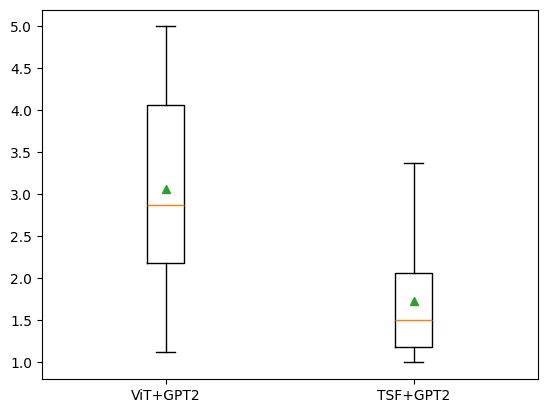
\includegraphics[width=0.5\linewidth]{boxplot.png}
    \caption{\textbf{キャプション生成モデルに対する評価の箱ひげ図}}
    図中の三角形はそのキャプション生成モデルに対する評価の平均値を表す.
    \label{fig:boxplot}
\end{figure}

\chapter{結論}
\label{conclusion}
\section{まとめ}

動画像キャプショニングモデルと文書埋め込みモデルを用いたプロンプトに対する生成動画像の追従度と人間の評価の相関を測定した結果,高い相関を得ることができず,既存手法と比較しても大きな差がなかった.実用化可能な性能とは言えないため,改良の必要がある.

\section{今後の予定}
今後の研究では上記の考察を検証するために,以下のことを実施し,プロンプトと生成動画像の関連性の評価に関する検討を続けていきたい.

\begin{quote}\begin{enumerate}
    \item プロンプトから画風や画角に関する記述,および固有名詞を排除した状態で実験を行う.
    \item 画風等の情報を生成できるようにキャプション生成モデルをファインチューニングする.
    \item 幅広い年齢層及び所属の人間からアンケートをとり,今回の実験の結果と比較する.
    \item 提案手法によるスコアの変動が小さい理由を調査する.
    \item コサイン類似度以外の方法による比較を試す.
\end{enumerate}\end{quote}

また,キャプション生成モデルについて追加のアンケートにより性能の評価を行った結果,性能が充分でないことが分かった.そのため,キャプション生成モデルを用いない別の評価方法についても考察する必要があると考える.

\chapter*{謝辞}
\addcontentsline{toc}{chapter}{謝辞}

本論文を作成するにあたり,指導教員である一関工業高等専門学校 未来創造工学科 情報・ソフトウェア系 助教 村上先生をはじめとして,ともに助言しあいながら研究に励んだ村上研究室の面々である同系5年 白沢,菅原,山崎や,アンケートにご協力くださった方々など,非常に多くの方々に多大なるご協力をいただきました.誠に感謝いたします.また,20年間支えてくださった両親にもこの場を借りて感謝の意を述べたいと思います.

\renewcommand{\bibname}{参考文献}
\addcontentsline{toc}{chapter}{参考文献}
\bibliographystyle{junsrt}
\bibliography{ref}

\end{document}